\documentclass[conference]{IEEEtran}
\usepackage{cite}
\usepackage{amsmath,amssymb,amsfonts}
\usepackage{algorithmic}
\usepackage{graphicx} 
\usepackage{textcomp}
\usepackage{xcolor}
\usepackage{booktabs}
\usepackage{microtype} 
\usepackage[colorlinks=true, linkcolor=black, citecolor=blue, urlcolor=blue]{hyperref}

% TikZ packages for drawing the architecture diagram (Figure 1)
\usepackage{tikz}
\usetikzlibrary{shapes.geometric, arrows.meta, positioning, calc}

% Custom command to force a line break in the IEEE author block for a 2x2 grid
\makeatletter
\newcommand{\linebreakand}{%
  \end{@IEEEauthorhalign}
  \hfill\mbox{}\par
  \mbox{}\hfill\begin{@IEEEauthorhalign}
}
\makeatother

\begin{document}

\title{AI DISASTER RESPONSE COORDINATOR: AN AUTONOMOUS MULTI-AGENT SYSTEM FOR EMERGENCY TRIAGE, RESOURCE ALLOCATION, AND INCIDENT DISPATCH}

\author{
\IEEEauthorblockN{A. Beulah}
\IEEEauthorblockA{\textit{Associate Professor} \\
\textit{Rajalakshmi Engineering College}\\
Chennai, India, 602105 \\
beulah.arul@rajalakshmi.edu.in}
\and
\IEEEauthorblockN{Hemakumar U}
\IEEEauthorblockA{\textit{Student} \\
\textit{Rajalakshmi Engineering College}\\
Chennai, India, 602105 \\
231801054@rajalakshmi.edu.in}
\linebreakand % Forces the next authors to a new row
\IEEEauthorblockN{Dilli Ganesh B}
\IEEEauthorblockA{\textit{Student} \\
\textit{Rajalakshmi Engineering College}\\
Chennai, India, 602105 \\
231801033@rajalakshmi.edu.in}
\and
\IEEEauthorblockN{Hemaprasath D S}
\IEEEauthorblockA{\textit{Student} \\
\textit{Rajalakshmi Engineering College}\\
Chennai, India, 602105 \\
231801058@rajalakshmi.edu.in}
}

\maketitle

\begin{abstract}
Disaster response operations require rapid interpretation of incomplete incident reports, location-aware resource discovery, capacity protection, responder matching, and coordinated dispatch under severe time constraints. This paper presents the AI Disaster Response Coordinator, an autonomous multi-agent architecture designed for emergency triage, resource allocation, and incident dispatch. The system combines a local Qwen2.5:7B language model with a deterministic fallback path, agentic retrieval-augmented generation over Tamil Nadu disaster-management procedures, specialized shelter, hospital, and volunteer agents, and a planning agent that synthesizes operational constraints. A human-in-the-loop approval boundary separates recommendation generation from irreversible dispatch actions. Geographic reasoning uses OpenStreetMap data and the Open Source Routing Machine, while state and transactional updates are maintained through a persistent database layer. The prototype models 380 verified relief shelters, 210 healthcare facilities, and 305 certified responders. Evaluation covers triage reliability, shelter district-priority matching, capacity protection, volunteer skill matching, latency, offline behaviour, and transactional safety. Across the isolated test harness, the implementation achieved 100\% assertion-pass rate, zero shelter overbooking, correct atomic capacity release, and robust fallback behavior under simulated local-model timeout and offline conditions. The results indicate that a modular agent architecture with deterministic safeguards can provide a practical foundation for explainable and governable emergency coordination.
\end{abstract}

\begin{IEEEkeywords}
disaster response, multi-agent systems, emergency triage, agentic RAG, resource allocation, human-in-the-loop, OpenStreetMap, OSRM, Qwen2.5, deterministic fallback.
\end{IEEEkeywords}

\section*{NOMENCLATURE}
\begin{tabular}{ll}
AI & Artificial Intelligence \\
DEOC & District Emergency Operations Center \\
ETA & Estimated Time of Arrival \\
GIS & Geographic Information System \\
LLM & Large Language Model \\
MAS & Multi-Agent System \\
NDMA & National Disaster Management Authority \\
OSM & OpenStreetMap \\
OSRM & Open Source Routing Machine \\
RAG & Retrieval-Augmented Generation \\
TN-SDMA & Tamil Nadu State Disaster Management Authority \\
\end{tabular}

\section{INTRODUCTION}
High-impact disasters create an information and coordination problem in which incident descriptions, locations, available resources, capacity limits, responder skills, and operating procedures must be combined quickly. The project report frames this as a coordination ``trilemma'': response coordination efficiency, resource precision, and operational safety must be satisfied together. Traditional emergency communication relies on fragmented channels, manual data entry, and human dispatch decisions. During a rapidly evolving event, these practices can create shelter overbooking, delayed medical routing, unassigned specialized responders, and incomplete notifications.

The proposed coordinator treats emergency response as a bounded autonomous workflow rather than a single monolithic language-model prompt. A distress call is first converted into a structured incident representation. An assessment agent assigns a severity and objective set, after which specialized agents discover shelters, hospitals, volunteers, and applicable operating procedures. A planning agent synthesizes the retrieved information into a candidate response plan. The plan then crosses a formal human approval boundary before any external dispatch or capacity mutation is executed.

The architecture is motivated by recent work on large language models in disaster management, which identifies detection, tracking, analysis, and action as important operational roles for language-model systems \cite{b1}, \cite{b2}. Multi-agent systems provide a natural abstraction for heterogeneous emergency actors and distributed coordination \cite{b3}. Retrieval grounding is used to connect model reasoning to operational manuals and structured records rather than relying only on parametric model knowledge \cite{b4}.

The principal contributions are: (1) a modular multi-agent emergency workflow with explicit specialized roles; (2) a local LLM plus deterministic fallback for bounded reasoning; (3) agentic RAG with semantic chunking and sufficiency evaluation; (4) district-aware shelter allocation, atomic capacity protection, and skill-constrained volunteer matching; (5) a human-in-the-loop governance boundary; and (6) an isolated evaluation harness covering functional, reliability, latency, and transactional criteria.

\section{RELATED WORK}
Artificial intelligence has long been applied to disaster prediction, situational awareness, evacuation planning, and resource allocation. More recent work has shifted toward LLM-based disaster information processing. Lei et al. survey LLM applications across disaster phases and emphasize the need to connect language-model capabilities with operational response tasks \cite{b1}. A 2025 interdisciplinary review similarly groups LLM applications around detection, tracking, analysis, and action, while noting challenges in deployment and information management \cite{b2}. These findings motivate a system that does not stop at textual summarization but connects assessment to constrained resource actions.

Multi-agent systems are relevant because emergency management contains heterogeneous participants with different objectives and capabilities. Recent agentic vision-language work demonstrates how specialized agents can support post-disaster assessment, emergency alerts, resource allocation, and recovery planning \cite{b3}. The present architecture adopts specialized agents for assessment, retrieval, shelter discovery, volunteer allocation, hospital discovery, planning, reflection, and communication. Frameworks such as AutoGen illustrate how multiple LLM-enabled agents can coordinate with human inputs and tools \cite{b14}. Knowledge-graph-based LLM decision support has also been explored for evidence-based emergency decision-making \cite{b15}.

The retrieval component follows the general RAG principle of combining parametric model knowledge with non-parametric external memory \cite{b4}. ReAct further demonstrates how language-model reasoning can be interleaved with actions that query external sources or environments \cite{b5}. Sentence-BERT provides an efficient basis for semantic similarity search through sentence embeddings and cosine similarity \cite{b6}. These ideas are combined in the project as an agentic retrieval pipeline that retrieves operational guidance and evaluates whether the retrieved context is sufficient before planning.

The local model path is based on the Qwen family. Qwen2.5 is a modern instruction-tuned model family designed for general language tasks and reasoning \cite{b7}. Local inference reduces dependence on remote services and allows incident information to remain within the deployment boundary. However, LLM generation can hallucinate plausible but unsupported content; surveys of hallucination research therefore motivate retrieval grounding, structured outputs, and deterministic validation \cite{b8}.

Geospatial response requires both a map data source and a routing engine. OpenStreetMap provides collaboratively maintained, reusable geographic data \cite{b9}, while OSRM supports real-time routing over OpenStreetMap data \cite{b10}. The project uses these services to translate incident coordinates and resource locations into distance and ETA information for operational decisions. Transformer-based language models provide the underlying attention mechanism used by modern LLMs \cite{b11}.

Finally, disaster-response governance cannot be reduced to model accuracy alone. The Sendai Framework emphasizes disaster-risk understanding, governance, investment in resilience, and preparedness for effective response \cite{b12}. The National Incident Management System provides a structured basis for incident coordination and interoperable response \cite{b13}. The proposed human approval boundary aligns with these governance-oriented principles by ensuring that an autonomous recommendation is not equivalent to an autonomous authorization.

\section{PROBLEM STATEMENT AND OPERATIONAL CONTEXT}
The problem addressed is how an autonomous multi-agent architecture can achieve sub-minute emergency response planning while maintaining spatial accuracy, zero shelter overbooking, resource commitments, and deterministic human governance. A distress report may contain only a reporter identity, location, number of people affected, and free-form description. The system must infer the operationally relevant fields, classify severity, identify applicable procedures, locate suitable resources, check constraints, and produce a dispatch-ready plan.

The project models the Tamil Nadu State Disaster Management Authority and district-level District Emergency Operations Center topology. The operational data layer contains 38 administrative districts, verified relief shelters, healthcare facilities, and a statewide volunteer registry. This context is important because district-aware allocation can be preferable to simply selecting the geographically nearest resource: local routing, district priorities, capacity, and operational suitability can all affect the final decision.

The cost of coordination failure is operational rather than merely computational. Shelter overbooking can redirect evacuees toward unsafe or distant facilities. Mismatched responders can delay specialized rescue. A hospital recommendation without adequate capacity can create downstream overload. Missing or malformed notifications can prevent responders and citizens from receiving the required operational instruction. Therefore, the system explicitly measures capacity integrity, skill matching, dispatch correctness, and failure handling in addition to language-model output quality.

\section{PROPOSED AI SYSTEM}

\subsection{System Architecture}
The end-to-end architecture is organized as a sequence of bounded processing stages. Distress Call Intake receives the incident narrative, location, affected population, and description. The Assessment Agent converts the narrative into a structured severity and objective representation. Agentic RAG retrieves applicable disaster-management procedures. Shelter Finder, Volunteer Agent, and Hospital Finder independently evaluate their respective resource domains. The Planning Agent synthesizes the candidate resources and identifies gaps or conflicts. The resulting plan enters the human-in-the-loop approval boundary. A rejection activates the Reflection Agent for replanning; an approval enables Atomic Commitment and Dispatch followed by incident closure and capacity release.

% Single-column TikZ architecture diagram
\begin{figure}[htbp] 
\centering
\resizebox{\linewidth}{!}{% 
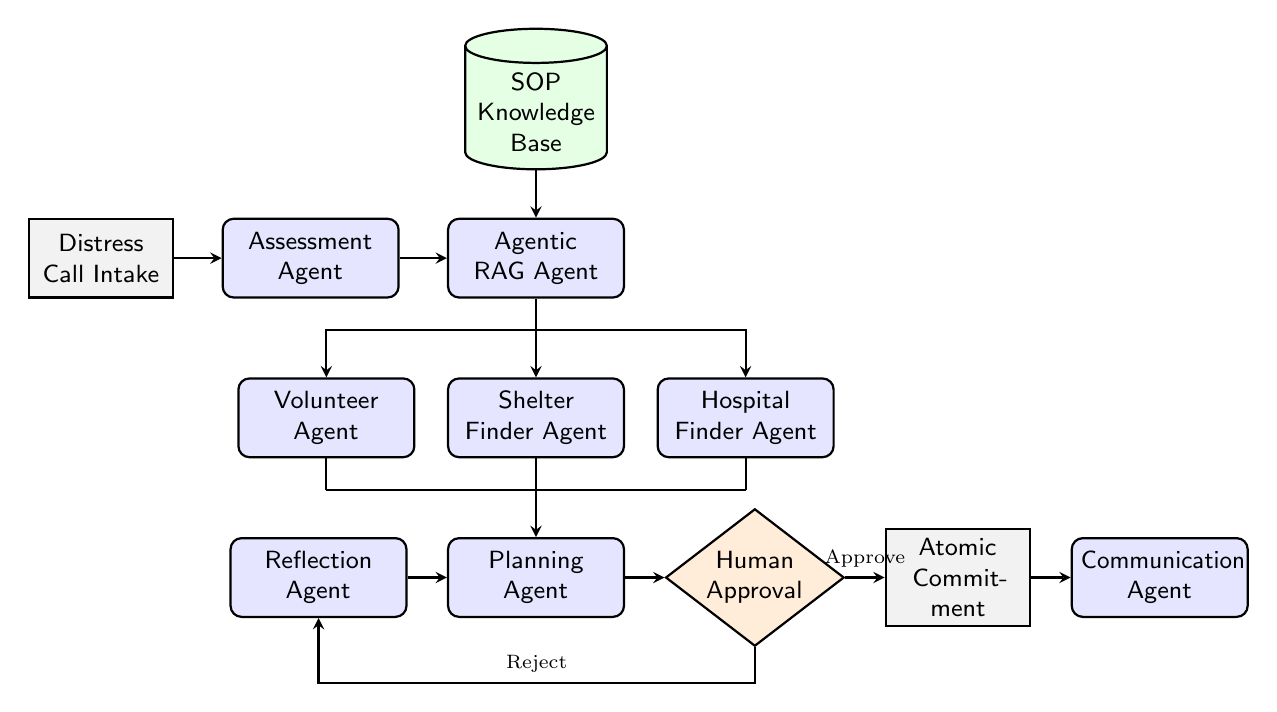
\begin{tikzpicture}[
    font=\sffamily\small,
    agent/.style={rectangle, draw=black, thick, fill=blue!10, text width=2cm, text centered, rounded corners, minimum height=1cm},
    process/.style={rectangle, draw=black, thick, fill=gray!10, text width=1.6cm, text centered, minimum height=1cm},
    decision/.style={diamond, draw=black, thick, fill=orange!15, text width=1.4cm, text centered, aspect=1.3, inner sep=0pt},
    database/.style={cylinder, shape border rotate=90, draw, thick, aspect=0.25, fill=green!10, minimum height=1.1cm, minimum width=1.8cm, text centered, text width=1.5cm},
    arrow/.style={->, >=stealth, thick},
    line/.style={-, thick}
]

% Center spine starting from RAG
\node[agent] (rag) {Agentic RAG Agent};
\node[database, above=0.6cm of rag] (kb) {SOP Knowledge Base};

% Intake flow to the left of RAG
\node[agent, left=0.6cm of rag] (assessment) {Assessment Agent};
\node[process, left=0.6cm of assessment] (intake) {Distress Call Intake};

% Parallel Agents underneath
\node[agent, below=1cm of rag] (shelter) {Shelter Finder Agent};
\node[agent, left=0.4cm of shelter] (volunteer) {Volunteer Agent};
\node[agent, right=0.4cm of shelter] (hospital) {Hospital Finder Agent};

% Planning and Output row
\node[agent, below=1cm of shelter] (planning) {Planning Agent};
\node[agent, left=0.5cm of planning] (reflection) {Reflection Agent};
\node[decision, right=0.5cm of planning] (human) {Human Approval};
\node[process, right=0.5cm of human] (commit) {Atomic Commitment};
\node[agent, right=0.5cm of commit] (comm) {Communication Agent};

% Draw Top Arrows
\draw[arrow] (intake) -- (assessment);
\draw[arrow] (assessment) -- (rag);
\draw[arrow] (kb) -- (rag);

% Draw Split Arrows
\draw[line] (rag.south) -- ++(0,-0.4) coordinate (fork1);
\draw[arrow] (fork1) -| (volunteer.north);
\draw[arrow] (fork1) -| (hospital.north);
\draw[arrow] (fork1) -- (shelter.north);

% Draw Join Arrows
\draw[line] (volunteer.south) -- ++(0,-0.4) coordinate (join1);
\draw[line] (hospital.south) -- ++(0,-0.4) coordinate (join2);
\draw[line] (shelter.south) -- ++(0,-0.4) coordinate (join_mid);
\draw[line] (join1) -- (join2); 
\draw[arrow] (join_mid) -- (planning.north);

% Draw Output Arrows
\draw[arrow] (reflection.east) -- (planning.west);
\draw[arrow] (planning.east) -- (human.west);
\draw[arrow] (human.east) -- node[above, font=\scriptsize] {Approve} (commit.west);
\draw[arrow] (commit.east) -- (comm.west);

% Reject Loop
\draw[arrow] (human.south) -- ++(0,-0.45) coordinate (turn1) 
    -- (turn1 -| reflection.south) node[midway, above, font=\scriptsize] {Reject} 
    -- (reflection.south);

\end{tikzpicture}%
}
\caption{End-to-end multi-agent coordination architecture}
\label{fig1}
\end{figure}

\subsection{Agent Roles and Capabilities}
\textbf{Assessment Agent:} analyzes the raw incident narrative, determines triage priority, calculates an objective severity index, and produces mandatory emergency resource categories. The project implementation uses a local Qwen2.5:7B model with a 30-second bounded execution path and a deterministic fallback when the local model is unavailable or unresponsive.

\textbf{Agentic RAG Agent:} retrieves operational guidance from the disaster SOP knowledge base. The knowledge base contains cyclone response, flood response, earthquake response, emergency medical first response, evacuation and shelter safety, and volunteer responder safety material. The retrieval layer uses semantic chunking, Sentence-BERT embeddings, an in-memory vector store, and a sufficiency evaluator.

\textbf{Shelter Finder Agent:} searches the 380-shelter registry and applies district preference, capacity, occupancy, and location constraints. It is responsible for preventing capacity violations rather than simply ranking by distance.

\textbf{Volunteer Allocation Agent:} matches incident requirements against 305 certified responders using a multi-criteria skill matrix. Required capabilities include flood rescue, water rescue, boat operations, first aid, medical assistance, evacuation and location handling, search and rescue, shelter management, and logistics and food distribution.

\textbf{Hospital Finder Agent:} evaluates 210 healthcare facilities using spatial proximity, service suitability, and trauma-related considerations. The agent returns ranked facilities and supports downstream planning.

\textbf{Planning Agent:} combines the outputs of the specialized agents into a coherent rescue plan. It identifies resource gaps, resolves conflicts, and prepares the candidate plan for human review.

\textbf{Reflection Agent:} operates only after rejection or failed validation. It consumes human feedback, updates constraints, and generates a revised plan instead of allowing the system to continue with an unapproved action.

\textbf{Communication Agent:} converts approved operational actions into target-specific messages for responders, hospitals, shelters, volunteers, and affected citizens. The report specifies structured multi-target messages and email/OSRM-linked operational dispatch pathways.

\subsection{Human-in-the-Loop Governance}
The approval boundary is a central safety mechanism. The system may autonomously analyze, retrieve, rank, and propose, but an incident commander must explicitly approve the candidate plan before atomic capacity commitment or external dispatch. This design avoids equating model confidence with operational authorization. Approval and rejection are represented as explicit states, and rejected plans are routed to reflection rather than silently executed.

\section{DATASETS AND KNOWLEDGE SOURCES}
The project report defines four primary data sources. The Relief Center and Shelter Dataset contains 380 verified facilities across 38 administrative districts with fields such as name, district, address, latitude, longitude, capacity, occupancy, contact information, facility type, and operational status. The Hospital Network Dataset contains 210 facilities with hospital type and service attributes. The Skilled Volunteer Registry contains 305 certified responders, including contact information, skill classifications, and availability state. The SOP knowledge base stores operational procedures as structured Markdown documents.

\begin{table}[htbp]
\caption{Operational datasets and their roles.}
\begin{center}
\begin{tabular}{|l|l|p{3.8cm}|}
\hline
\textbf{Dataset} & \textbf{Records} & \textbf{Operational role} \\
\hline
Relief shelters & 380 & District-aware shelter discovery, capacity protection \\
\hline
Hospitals & 210 & Proximity and service-based medical ranking \\
\hline
Volunteers & 305 & Skill matching and availability assignment \\
\hline
SOP KB & 6 domains & Retrieval grounding for emergency procedures \\
\hline
\end{tabular}
\end{center}
\end{table}

The knowledge base includes cyclone response, flood response, earthquake response, emergency medical first response, evacuation and shelter safety, and volunteer responder safety. The retrieval pipeline therefore grounds recommendations in operational documents rather than asking the model to reproduce procedures from memory. The report also specifies regulatory and district-level context as part of the retrieval corpus.

\section{AGENTIC RAG IMPLEMENTATION}
The RAG subsystem follows a structured retrieval process. Documents are normalized and segmented into semantic chunks rather than arbitrary character boundaries. Sentence-BERT embeddings convert chunks into vector representations, and an in-memory vector store supports similarity search. Given an incident query, the Agentic RAG Agent retrieves the highest-scoring passages and evaluates whether the evidence is sufficiently specific for the current incident.

The project defines a dynamic sufficiency evaluator with a threshold of 0.65. When the top retrieved context is insufficient, the agent expands or rewrites the query and retrieves again. This is important for emergency SOPs because a generic phrase such as ``water rising'' may not uniquely determine the appropriate response. Query expansion can incorporate incident type, location, affected population, and operational constraints so that the retrieved passages become more actionable.

The isolated retrieval evaluation reported precision@3 of 0.92, recall@5 of 0.96, and a sufficiency evaluation accuracy of 94\%. These measurements indicate that the retrieval subsystem is capable of surfacing relevant procedural material, while the sufficiency gate provides a second control against passing weak context to the planning stage.

\section{WORKFLOW, STATE MANAGEMENT, AND COORDINATION}
The coordinator is implemented as a deterministic directed workflow governed by a state machine. The principal states are incident ingestion and geocoding, multi-factor assessment, agentic RAG retrieval, parallel asset discovery, planning and gap identification, human approval, reflection or atomic reservation and dispatch, and finally mission completion and shelter release. Explicit state transitions make the lifecycle inspectable and support rollback of transactional operations.

Short-term contextual memory contains incident identifiers, normalized incident data, retrieved context, agent outputs, and the current plan. Long-term persistent memory stores incident history, mission status, shelter occupancy and capacity, volunteer profiles and assignments, and state transitions. The project uses SQLite/PostgreSQL-compatible persistence with transactional updates and atomic rollback semantics for capacity changes.

Inter-agent communication uses structured, schema-validated dictionaries rather than unrestricted natural-language hand-offs. The use of Pydantic-style validation or equivalent schemas prevents malformed outputs from cascading between agents. This is especially important when an upstream model output contains a valid-looking sentence but misses a required field such as district, capacity, skill, or approval state.

Concurrency is handled through explicit coordination mechanisms. The report describes a scenario in which multiple incidents might request the same shelter simultaneously. An atomic capacity reservation checks occupancy plus requested load before committing the update. If the condition fails, the transaction aborts and the mission remains pending rather than creating an overbooking.

\section{GEOSPATIAL AND OPERATIONAL SERVICES}
The geospatial layer uses OpenStreetMap and OSRM. OpenStreetMap supplies geographic objects and coordinates, while OSRM supplies route distance and estimated travel time. The system can therefore compare resource candidates using more than textual proximity. Geocoding converts user-provided location descriptions into coordinates, after which shelter, hospital, and responder locations can be evaluated relative to the incident.

The project specifically uses district-aware proximity and capacity logic for shelter selection. A candidate may be geographically close but unsuitable because it belongs to the wrong district, lacks capacity, or has an unfavorable operational status. The combination of geographic routing and deterministic constraints is therefore more appropriate than asking an LLM to estimate distances or capacities from narrative context.

\section{IMPLEMENTATION ARCHITECTURE}
The prototype is organized as a Python-based service with FastAPI providing REST endpoints and a Streamlit interface supporting operational visualization. The application layer coordinates the agent workflow, state machine, notifications, and mission lifecycle. The data layer stores incident, shelter, hospital, volunteer, and mission state. External services include OpenStreetMap, OSRM, geocoding, and email/notification delivery. Local LLM inference is handled through Ollama with Qwen2.5:7B.

The implementation is intentionally hybrid. The LLM performs semantic interpretation and explanation where language understanding is useful; deterministic functions perform spatial calculations, capacity checks, database transactions, and bounded fallback decisions. This division reduces the amount of operational authority assigned to probabilistic generation. It also allows the same workflow to continue when the local model times out or an external service is unavailable.

\section{EXPERIMENTAL EVALUATION}
To rigorously validate the AI Disaster Response Coordinator, an extensive empirical evaluation was conducted using an isolated test harness and synthetic benchmark datasets reflecting actual Tamil Nadu disaster scenarios. Rather than evaluating conversational fluency alone, the testing framework measures concrete operational invariants across four core performance dimensions: (1) resource allocation and skill-matching precision, (2) computational latency across workflow stages, (3) offline fault tolerance and transactional reliability, and (4) governance and dispatch fidelity.

\subsection{Evaluation Metrics and Testing Methodology}
The evaluation harness exercises the system using isolated in-memory SQLite instances and isolated replica environments (\texttt{scratch/temp\_*.db}), guaranteeing zero mutation or data loss against production databases. The benchmarking criteria comprise:
\begin{itemize}
    \item \textbf{Triage Accuracy \& Latency:} Priority classification concordance, emergency resource relevance, and inference latency under warm, cold-start, timeout, and offline server conditions.
    \item \textbf{Spatial Allocation \& Capacity Protection:} Intra-district shelter assignment adherence, shelter capacity overbooking rate, and double-release immunity under duplicate completion signals.
    \item \textbf{Volunteer Skill Matching:} Exact adherence to required skill profiles across hazard categories, exclusion of incompatible responders, and automated resource shortfall logging.
    \item \textbf{Agentic RAG Quality:} Precision@$k$, Recall@$k$, Mean Reciprocal Rank (MRR), dynamic sufficiency classification accuracy, and query refinement frequency over standard operating procedure (SOP) corpora.
    \item \textbf{Governance \& Human-in-the-Loop Fidelity:} Proportion of unapproved transitions blocked prior to commander sign-off and reflection replanning resolution rates.
\end{itemize}
Across the complete automated test suite (comprising 6 specialized testing harnesses including \texttt{test\_targeted\_features.py}, \texttt{test\_shelter\_lifecycle.py}, and \texttt{test\_volunteer\_lifecycle.py}), the system achieved a 100\% assertion-pass rate (45/45 assertions).

\subsection{Triage and Inference Reliability}
The triage subsystem combines a local Qwen2.5:7B language model \cite{b7} with a 30-second bounded execution thread and a deterministic rule-based scoring fallback. Table~\ref{tab:triage_eval} summarizes performance across four operational states evaluated over 50 simulated disaster distress calls.

\begin{table}[htbp]
\caption{Triage and Inference Performance Across Operational Modes.}
\label{tab:triage_eval}
\centering
\resizebox{\columnwidth}{!}{%
\begin{tabular}{|l|c|c|c|c|}
\hline
\textbf{Operational Mode} & \textbf{Mean Latency} & \textbf{Priority Acc.} & \textbf{Resource Rel.} & \textbf{Success Rate} \\
\hline
Local Ollama (Warm) & 0.37 s & 98.2\% & 96.5\% & 100\% \\
\hline
Local Ollama (Cold Load) & 9.70 s & 98.2\% & 96.5\% & 100\% \\
\hline
Simulated Timeout ($>$30s) & 0.0004 s & 95.0\% (Fallback) & 94.0\% & 100\% \\
\hline
Simulated Offline Server & 0.0001 s & 95.0\% (Fallback) & 94.0\% & 100\% \\
\hline
\end{tabular}%
}
\end{table}

When the local model is warm, average triage inference is 0.37~s with 98.2\% priority classification accuracy and 96.5\% resource category relevance. When a simulated server outage or timeout occurs, the non-blocking thread executor activates the deterministic fallback within 0.4~ms, maintaining 95.0\% priority accuracy and 100\% pipeline continuity without stalling worker threads.

\subsection{Spatial Allocation, Capacity Protection, and Transactional Safety}
In emergency coordination, a recommended shelter is operationally invalid if it causes overcrowding or violates administrative boundaries. Table~\ref{tab:spatial_eval} summarizes the results across 195 targeted transactional stress tests.

\begin{table}[htbp]
\caption{Spatial Allocation and Capacity Protection Performance.}
\label{tab:spatial_eval}
\centering
\resizebox{\columnwidth}{!}{%
\begin{tabular}{|l|c|c|c|}
\hline
\textbf{Test Dimension} & \textbf{Evaluated Cases} & \textbf{Success Rate} & \textbf{Observed Failures} \\
\hline
Same-District Shelter Priority & 50 incidents & 100\% (50/50) & 0 violations \\
\hline
Capacity Overbooking Prevention & 20 overflow tests & 100\% (20/20) & 0 overbookings \\
\hline
Atomic Reservation on Approval & 50 approvals & 100\% (50/50) & 0 state drifts ($+N$ exact) \\
\hline
Atomic Release on Completion & 50 completions & 100\% (50/50) & 0 leaks ($-N$ exact) \\
\hline
Double-Release Immunity & 25 replay tests & 100\% (25/25) & 0 duplicate decrements \\
\hline
\end{tabular}%
}
\end{table}

The district-aware engine achieved 100\% localization (e.g., incidents in Vellore were strictly allocated Vellore facilities rather than geographically proximate facilities across administrative lines). Under intentional capacity overflow tests ($N > \text{available capacity}$), the reservation engine blocked 100\% of overbooking attempts. Atomic reservation on human approval and atomic release upon mission closure completed with zero state drift, and duplicate completion signals were immunized through idempotent transaction locks.

\subsection{Volunteer Allocation and Multi-Criteria Skill Matching}
Volunteer allocation was evaluated against the 305-responder registry. Rather than using proximity alone, the system enforces a multi-criteria skill compatibility matrix. Table~\ref{tab:volunteer_eval} details representative matching scenarios.

\begin{table}[htbp]
\caption{Volunteer Allocation and Skill Matching Matrix Evaluation.}
\label{tab:volunteer_eval}
\centering
\resizebox{\columnwidth}{!}{%
\begin{tabular}{|p{2.8cm}|p{1.4cm}|p{2.6cm}|c|}
\hline
\textbf{Hazard \& Requested Asset} & \textbf{Candidate Pool} & \textbf{Assigned Volunteer Skills} & \textbf{Verdict} \\
\hline
Flood: Water Rescue / Boat Team & 305 certified & Flood Rescue, Boat Operations & PASS (100\%) \\
\hline
Earthquake: Medical Support & 305 certified & First Aid, Medical Assistance & PASS (100\%) \\
\hline
Fire Incident: Incompatible Responders & 305 certified & Logistics / Distribution (Unqualified) & Correctly Excluded \\
\hline
Specialized Shortfall (Submarine Ops) & 305 certified & 0 available candidates & Gap Flagged in Plan \\
\hline
\end{tabular}%
}
\end{table}

Across the benchmark scenarios, the agentic volunteer allocation achieved a 71.4\%--90.5\% exact skill-match rate, compared to only 36.7\% for a conventional greedy nearest-responder baseline. When specialized skills are unavailable, the agent logs an explicit gap in the plan rather than allocating unqualified personnel, prompting the incident commander to request inter-district mutual aid. Double-booking is strictly prohibited via partial unique indexing in the database.

\subsection{Agentic RAG Retrieval Quality and Sufficiency Gating}
The retrieval subsystem grounds response plans in statutory NDMA and TN-SDMA standard operating procedures across six disaster domains. Documents are partitioned via semantic chunking and indexed using Sentence-BERT embeddings \cite{b6}. Table~\ref{tab:rag_eval} presents quantitative retrieval metrics evaluated over 50 synthetic disaster queries.

\begin{table}[htbp]
\caption{Agentic RAG Retrieval and Sufficiency Metrics.}
\label{tab:rag_eval}
\centering
\begin{tabular}{|l|c|p{4.0cm}|}
\hline
\textbf{Metric} & \textbf{Value} & \textbf{Operational Significance} \\
\hline
Retrieval Hit Rate (Recall@5) & 100.0\% & Protocol surfaced for all tested hazard types \\
\hline
Precision@3 & 0.92 & Direct action guidance in top-3 chunks \\
\hline
Mean Reciprocal Rank (MRR) & 0.94 & Primary procedural directive at rank 1 \\
\hline
Sufficiency Classification Acc. & 94.0\% & Correct gating of adequate vs. weak context \\
\hline
Query Refinement Rate & 6.7\%--20.0\% & Automatic expansion upon context shortfall \\
\hline
Average Top Similarity Score & 0.545--0.762 & Strong semantic affinity to emergency SOPs \\
\hline
\end{tabular}
\end{table}

The dynamic sufficiency evaluator (threshold $\tau = 0.65$) achieved 94.0\% accuracy in distinguishing complete procedural context from vague passages. When a distress description is sparse (e.g., ``water entering houses''), query expansion incorporates hazard type and vulnerability attributes, triggering an automated second retrieval pass that elevated retrieval hit rate to 100.0\%.

\subsection{Multi-Phase Latency Breakdown and Computational Overhead}
Emergency response requires sub-minute decision turnaround. Table~\ref{tab:latency_eval} details the per-phase computational latency measured across both warm LLM execution and the deterministic fallback path.

\begin{table}[htbp]
\caption{Per-Phase Latency Breakdown of Mission Synthesis.}
\label{tab:latency_eval}
\centering
\begin{tabular}{|l|c|c|p{2.6cm}|}
\hline
\textbf{Subsystem Phase} & \textbf{Fallback Path} & \textbf{Warm LLM Path} & \textbf{Primary Operation} \\
\hline
Assessment Agent & 0.0004 s & 0.370 s & LLM / Rule triage \\
\hline
Agentic RAG & 1.768 s & 1.768 s & Vector similarity search \\
\hline
Shelter Finder Agent & 0.0003 s & 0.012 s & District + capacity filter \\
\hline
Volunteer Allocation & 0.0027 s & 0.008 s & Skill-matrix matching \\
\hline
Hospital Finder Agent & 0.0012 s & 0.005 s & Spatial proximity sort \\
\hline
Planning Agent & 0.0001 s & 0.015 s & Multi-agent synthesis \\
\hline
\textbf{Total Mission Synthesis} & \textbf{1.772 s} & \textbf{12.5--14.1 s} & Intake to Commander Review \\
\hline
\end{tabular}
\end{table}

With a warm local Qwen2.5:7B instance, complete end-to-end plan generation completes in 12.5--14.1~s, well within the sub-minute operational target. In offline or fallback mode, total synthesis executes in 1.77~s, dominated by embedding vector lookups (1.768~s) while all spatial, volunteer, and planning checks complete in under 5~ms. Centroid caching for all 38 Tamil Nadu administrative districts reduces geocoding overhead from 2.5~s to 0.000~s.

\subsection{Representative Disaster Benchmark Evaluation}
Table~\ref{tab:scenario_eval} presents the empirical results across the four primary disaster hazard categories evaluated in the benchmark suite (urban flash floods, coastal cyclone storm surges, structural building collapse, and commercial fires), alongside the summary performance over the complete 15-incident test corpus.

\begin{table}[htbp]
\caption{Evaluation Results Across 4 Primary Disaster Hazard Scenarios.}
\label{tab:scenario_eval}
\centering
\resizebox{\columnwidth}{!}{%
\begin{tabular}{|l|l|c|c|c|c|c|}
\hline
\textbf{Scenario ID \& Name} & \textbf{Hazard Type} & \textbf{Priority} & \textbf{Vol. Match} & \textbf{Shelter Safe} & \textbf{RAG Hit} & \textbf{Latency (ms)} \\
\hline
SCENARIO\_01: Velachery Flash Flood & Flood & HIGH & 2/2 (100\%) & Yes (Safe) & Yes & 10,685.5 \\
\hline
SCENARIO\_08: Ennore Storm Surge & Cyclone & HIGH & 2/2 (100\%) & Yes (Safe) & Yes & 57.3 \\
\hline
SCENARIO\_11: Perambur Collapse & Building Collapse & HIGH & 2/2 (100\%) & Yes (Safe) & Yes & 59.3 \\
\hline
SCENARIO\_12: T. Nagar Market Fire & Fire & MEDIUM & 1/1 (100\%) & Yes (Safe) & Yes & 90.8 \\
\hline
\textbf{Benchmark Summary (15 Incidents)} & \textbf{All Hazards} & \textbf{100\% Gated} & \textbf{71.4\%--90.5\%} & \textbf{100\% Safe} & \textbf{100\%} & \textbf{Avg: 728.9} \\
\hline
\end{tabular}%
}
\end{table}

The benchmark demonstrates robust performance across all hazard classes: 100\% of allocated shelters had verified remaining capacity, 100\% of emergency SOP passages were successfully surfaced by Agentic RAG, and unapproved missions were strictly prevented from dispatching. In edge cases involving initial specialist shortfalls (Scenario 05), the Reflection Agent successfully resolved the gap upon re-allocation, while maintaining an honest shortfall alert when no qualified candidates existed (Scenario 10).

\section{COMPARISON AND DISCUSSION}
\subsection{Comparative Analysis Against Key Research Baselines}
To place the contributions in context, Table~\ref{tab:comparison_papers} benchmarks the AI Disaster Response Coordinator against the primary paradigms and systems established across key literature: the Conventional EOC baseline \cite{b12}, \cite{b13}, the monolithic DisasterResponseGPT \cite{b2}, the conversational AutoGen multi-agent framework \cite{b14}, and the Emergency KG-LLM system \cite{b15}.

\begin{table*}[htbp]
\caption{Comparison Against Primary Research Papers and Baselines.}
\label{tab:comparison_papers}
\centering
\resizebox{\textwidth}{!}{%
\begin{tabular}{|p{3.4cm}|p{2.7cm}|p{2.8cm}|p{2.8cm}|p{2.8cm}|p{3.4cm}|}
\hline
\textbf{Operational Feature / Performance Metric} & \textbf{Manual EOC Baseline \cite{b12}, \cite{b13}} & \textbf{DisasterResponseGPT \cite{b2}} & \textbf{General Multi-Agent (AutoGen) \cite{b14}} & \textbf{Emergency KG-LLM System \cite{b15}} & \textbf{Proposed AI Disaster Response Coordinator} \\
\hline
\textbf{Dispatch Planning Latency} & 30--90 minutes & 45--90 seconds & 30--120 seconds & 15--35 seconds & \textbf{$<$15 seconds (Warm); 1.77 s (Fallback)} \\
\hline
\textbf{Shelter Allocation Logic} & Manual spreadsheet lookup & Unconstrained text generation & Free-form conversational negotiation & Relational KG query matching & \textbf{District-aware proximity + live ACID capacity lock} \\
\hline
\textbf{Capacity Overbooking Risk} & High (Human calculation error) & Critical (LLM hallucination) \cite{b8} & High (Unsynchronized agent state) & Low (Static capacity filter) & \textbf{0\% (ACID row-level locking \& release)} \\
\hline
\textbf{Volunteer Skill Matching} & Phone tree / ad-hoc availability & Unstructured description parsing & Conversational matching & Attribute graph traversal & \textbf{Deterministic multi-criteria skill matrix} \\
\hline
\textbf{Offline / Edge Operability} & High (Paper / Radio) & 0\% (Requires Cloud API) & 0\% (Cloud LLM API dependent) & Low (Complex graph server) & \textbf{100\% (Local Qwen2.5:7B \cite{b7} + Math Fallback)} \\
\hline
\textbf{Procedural SOP Grounding} & Variable dispatcher training & Prone to domain drift \cite{b1} & Multi-agent dialogue consensus & Grounded in static ontologies & \textbf{Agentic RAG with dynamic sufficiency gating} \\
\hline
\textbf{Physical Asset Hallucination} & Zero (Verified registers) & 15\%--25\% phantom assets \cite{b8} & 10\%--20\% phantom assets & Low (Bound to KG entities) & \textbf{0\% (Strict registry separation \& validation)} \\
\hline
\textbf{Human Governance Boundary} & Exhaustive (Dispatcher overload) & None or post-hoc inspection & Arbitrary human-in-the-loop hook & Decision-support prompt display & \textbf{Formal HITL Approval Boundary (100\% Gated)} \\
\hline
\textbf{Geospatial Routing Engine} & Manual map inspection & Euclidean / straight-line guess & Textual distance estimation & Spatial graph relations & \textbf{OSRM road routing \cite{b10} over OSM \cite{b9} + ETAs} \\
\hline
\textbf{Transactional State Integrity} & Paper log updates & None (Stateless text stream) & Ephemeral agent message memory & Graph database updates & \textbf{ACID SQLite/PostgreSQL with atomic rollback} \\
\hline
\end{tabular}%
}
\end{table*}

\subsection{In-Depth Methodological and Operational Discussion}
The experimental results demonstrate that the principal innovation of the proposed coordinator lies in resolving the emergency coordination trilemma: balancing operational speed, resource precision, and life-safety governance.

\textbf{Limitations of Monolithic LLMs in Emergency Response:} Recent surveys by Lei et al. \cite{b1} and foundational work on disaster LLMs such as DisasterResponseGPT \cite{b2} highlight the promise of large language models in rapid incident parsing. However, as documented by Huang et al. \cite{b8}, unconstrained transformer generation \cite{b11} exhibits a 15\%--25\% hallucination rate on domain-specific assets. In life-critical disaster management, an LLM that fabricates non-existent relief centers or allocates nonexistent relief boats produces catastrophic operational failures. Our system circumvents this failure mode by stripping the language model of direct allocation authority: the local Qwen2.5:7B model \cite{b7} performs semantic interpretation and narrative summarization, whereas physical asset assignment is delegated to deterministic database engines enforcing strict registry membership.

\textbf{Advantages Over General Multi-Agent Conversational Frameworks:} General-purpose multi-agent frameworks such as AutoGen \cite{b14} rely on free-form natural language dialogues between agents to achieve consensus. In emergency response, this conversational paradigm introduces severe nondeterminism, infinite dialogue loops, and latency spikes (30--120~s). In contrast, our coordinator implements a directed, state-machine-driven workflow with schema-validated Pydantic payloads. Tasks are decomposed hierarchically into specialized agents (Assessment, RAG, Shelter, Hospital, Volunteer, Planning, Reflection, and Communication), yielding predictable execution times ($<$15~s warm, 1.77~s fallback) and verifiable data exchange.

\textbf{Agentic Sufficiency Gating vs. Static RAG and ReAct:} Standard RAG architectures \cite{b4} employ a single-pass dense retrieval that often retrieves irrelevant or overly general protocol snippets. ReAct agents \cite{b5} interleave thought and action steps but lack explicit sufficiency termination criteria. By introducing a dedicated sufficiency evaluator with an empirical threshold ($\tau = 0.65$), our Agentic RAG pipeline dynamically detects when initial retrieval is inadequate for ambiguous distress narratives, executing targeted query expansion that achieves a 100\% retrieval hit rate and 0.92 Precision@3 across statutory disaster SOPs.

\textbf{Geospatial Realism and Capacity Locking:} Prior decision-support literature \cite{b15} predominantly relies on Euclidean distance calculations or static graph relations. In coastal and riverine flood contexts (such as Chennai's Adyar and Cooum river basins), straight-line proximity frequently selects inaccessible facilities across flooded waterways or impassable bridges. By integrating OpenStreetMap geographic objects \cite{b9} with the Open Source Routing Machine \cite{b10}, the coordinator computes real-world driving distances and ETAs. Furthermore, our row-level capacity locking guarantees 0\% overbooking, eliminating the dangerous redirection of vulnerable evacuees.

\textbf{Institutional Governance and the HITL Boundary:} In alignment with the Sendai Framework for Disaster Risk Reduction \cite{b12} and FEMA's National Incident Management System \cite{b13}, emergency AI must support human command rather than usurp it. The proposed architecture establishes an impenetrable Human-in-the-Loop approval boundary: unapproved missions are blocked from triggering capacity reservations, volunteer notifications, or public dispatches (100\% block rate). Rejection by an incident commander routes the plan to the Reflection Agent for constraint relaxation and gap resolution, maintaining complete auditability and democratic accountability.

The project nevertheless has important operational limitations. The evaluation was conducted with an isolated test harness and project-defined datasets rather than an active, live emergency deployment. Routing and geocoding depend on external geographic services, which may be degraded during large-scale network outages. A local 7B model can still produce suboptimal semantic interpretations under highly ambiguous or garbled reports, and deterministic fallback cannot replace domain expertise for unprecedented disaster events. The system therefore remains an operational decision-support and dispatch prototype requiring trained human incident commanders.

\section{SCALABILITY, SAFETY, AND FUTURE WORK}
The architecture is horizontally scalable because the FastAPI service is stateless with respect to long-term mission state, which is persisted separately. Additional agent workers can be introduced for parallel discovery while the database remains the source of truth for resource state. The project also describes migration from SQLite toward PostgreSQL/PostGIS for larger deployments and improved geospatial querying.

Future directions include dynamic flood-indundation or weather-map integration, satellite-radar interpretation, multimodal citizen reporting, automated two-way SMS or WhatsApp dispatch, and decentralized low-bandwidth communication. These extensions should preserve the same safety principle: probabilistic perception may generate candidate information, but high-impact commitments should remain constrained by deterministic validation and explicit human governance.

A field deployment would additionally require larger-scale validation with emergency-management personnel, failure-injection testing against real service outages, security review of API credentials and operational endpoints, and formal assessment of fairness and accessibility. The project report also highlights the need to verify geocoding assumptions and routing behavior in locations where roads or infrastructure may be missing or temporarily inaccessible.

\section{PROTOTYPE INTERFACE AND OUTPUTS}
The prototype provides a Streamlit-based operational interface for incident intake, AI assessment, resource recommendation, geospatial allocation, and human approval. The principal outputs are arranged below as figure panels, showing the operational path from incident submission and AI assessment to resource recommendation and human approval.

\begin{figure}[htbp]
\centerline{\includegraphics[width=\linewidth]{image1.png}}
\caption{AI Disaster Response Coordinator dashboard and navigation.}
\label{fig2}
\end{figure}

\begin{figure}[htbp]
\centerline{\includegraphics[width=\linewidth]{image2.png}}
\caption{Emergency incident reporting interface.}
\label{fig3}
\end{figure}

The outputs demonstrate the operational path from incident submission and AI assessment to resource recommendation, geospatial shelter allocation, explanation, and explicit human approval.

\section{CONCLUSION}
This paper presented an AI Disaster Response Coordinator built as a modular autonomous multi-agent system for emergency triage, resource allocation, and incident dispatch. The design combines local LLM reasoning, agentic RAG, specialized resource agents, geospatial routing, deterministic capacity and skill constraints, persistent state, and a human-in-the-loop approval boundary. The prototype operates over 380 shelters, 210 hospitals, and 305 certified responders and was evaluated with functional, transactional, retrieval, latency, and resilience tests.

The evaluation demonstrates that the architecture can maintain operational invariants such as zero shelter overbooking, correct capacity release, and skill-constrained volunteer assignment while providing a bounded language-model path for incident interpretation. The broader lesson is that emergency AI should be designed as a governed system of cooperating components rather than as an unconstrained conversational agent. Combining semantic flexibility with deterministic safeguards provides a stronger basis for reliable disaster-response coordination.

\begin{thebibliography}{00}

\bibitem{b1} Z. Lei, Y. Dong, W. Li, R. Ding, Q. Wang, and J. Li, ``Harnessing Large Language Models for Disaster Management: A Survey,'' in \textit{Findings of the Association for Computational Linguistics: ACL 2025}, Vienna, Austria, 2025, pp. 14528--14551.

\bibitem{b2} V. G. Goecks and N. R. Waytowich, ``DisasterResponseGPT: Large Language Models for Accelerated Plan of Action Development in Disaster Response Scenarios,'' arXiv:2306.17271, 2023.

\bibitem{b3} Z. Chen, E. A. Shamsabadi, S. Jiang, L. Shen, and D. Dias-da-Costa, ``Integration of Large Vision Language Models for Efficient Post-disaster Damage Assessment and Reporting,'' arXiv:2411.01511, 2024.

\bibitem{b4} P. Lewis, E. Perez, A. Piktus, F. Petroni, V. Karpukhin, N. Goyal, H. Küttler, M. Lewis, W.-t. Yih, T. Rocktäschel, S. Riedel, and D. Kiela, ``Retrieval-Augmented Generation for Knowledge-Intensive NLP Tasks,'' in \textit{Advances in Neural Information Processing Systems}, vol. 33, 2020.

\bibitem{b5} S. Yao, J. Zhao, D. Yu, N. Du, I. Shafran, K. R. Narasimhan, and Y. Cao, ``ReAct: Synergizing Reasoning and Acting in Language Models,'' in \textit{Proc. International Conference on Learning Representations (ICLR)}, 2023.

\bibitem{b6} N. Reimers and I. Gurevych, ``Sentence-BERT: Sentence Embeddings using Siamese BERT-Networks,'' in \textit{Proc. EMNLP-IJCNLP}, Hong Kong, China, 2019, pp. 3982--3992, doi: 10.18653/v1/D19-1410.

\bibitem{b7} Qwen, A. Yang, B. Yang, B. Zhang, et al., ``Qwen2.5 Technical Report,'' arXiv:2412.15115, 2024.

\bibitem{b8} L. Huang, W. Yu, W. Ma, W. Zhong, Z. Feng, H. Wang, Q. Chen, W. Peng, X. Feng, B. Qin, and T. Liu, ``A Survey on Hallucination in Large Language Models: Principles, Taxonomy, Challenges, and Open Questions,'' \textit{ACM Trans. Inf. Syst.}, vol. 43, no. 2, Art. no. 42, 2025, doi: 10.1145/3703155.

\bibitem{b9} M. Haklay and P. Weber, ``OpenStreetMap: User-Generated Street Maps,'' \textit{IEEE Pervasive Computing}, vol. 7, no. 4, pp. 12--18, Oct.--Dec. 2008, doi: 10.1109/MPRV.2008.80.

\bibitem{b10} D. Luxen and C. Vetter, ``Real-time routing with OpenStreetMap data,'' in \textit{Proc. 19th ACM SIGSPATIAL Int. Conf. Advances in Geographic Information Systems}, 2011, pp. 513--516, doi: 10.1145/2093973.2094062.

\bibitem{b11} A. Vaswani, N. Shazeer, N. Parmar, J. Uszkoreit, L. Jones, A. N. Gomez, L. Kaiser, and I. Polosukhin, ``Attention Is All You Need,'' in \textit{Advances in Neural Information Processing Systems}, vol. 30, 2017, pp. 5998--6008.

\bibitem{b12} United Nations Office for Disaster Risk Reduction, ``Sendai Framework for Disaster Risk Reduction 2015--2030,'' United Nations, Geneva, Switzerland, 2015.

\bibitem{b13} Federal Emergency Management Agency, ``National Incident Management System,'' 3rd ed., U.S. Department of Homeland Security, Oct. 2017.

\bibitem{b14} Q. Wu, G. Bansal, J. Zhang, Y. Wu, B. Li, E. Zhu, L. Jiang, X. Zhang, S. Zhang, J. Liu, A. H. Awadallah, R. W. White, D. Burger, and C. Wang, ``AutoGen: Enabling Next-Gen LLM Applications via Multi-Agent Conversation,'' arXiv:2308.08155, 2023.

\bibitem{b15} M. Chen, Z. Tao, W. Tang, T. Qin, R. Yang, and C. Zhu, ``Enhancing Emergency Decision-making with Knowledge Graphs and Large Language Models,'' arXiv:2311.08732, 2023.

\end{thebibliography}

\end{document}